%%%%%%%%%%%%%%%%%%%%%%%%%%%%%%%%%%%%%%%%%%%%%%%%%%%%%%%%%%%%%%%%%%%%%%%%%%%%%%%%%%%%%%%%%%%%%%%%%%%%%%
%
%   Filename    : chapter_1.tex 
%
%   Description : This file will contain your Research Description.
%                 
%%%%%%%%%%%%%%%%%%%%%%%%%%%%%%%%%%%%%%%%%%%%%%%%%%%%%%%%%%%%%%%%%%%%%%%%%%%%%%%%%%%%%%%%%%%%%%%%%%%%%%

\chapter{Research Description}
\label{sec:researchdesc}    %--note: labels help you with hyperlink editing (using your IDE)

\begin{comment}
Make sure to write a preamble for each chapter, i.e., a short description of what each chapter contains before 
the first section within the chapter.  The preamble can be written in about two to three sentences.
\end{comment}

\section{Overview of the Current State of Technology}
\label{sec:overview}

%
%   NOTE: You have to delete/replace the unnecessary paragraphs with your own text.
%

Telediagnosis is a diagnosis that occurs at a remote location and is based on the evaluation of data transmitted from devices that monitor the patient \cite{telediagnosis}. Computer systems connecting patients, midwives and doctors assist the telediagnosis process. For maximized collaboration and effectiveness, a good system design must adjust to the current business process the doctors and midwives are familiar with and not the other way around. The system must be a convenient tool for the people using it. Since the doctors and midwives are adapted to traditional ways such as writing on paper or vocal narration, it is best if they are not forced to divert from what they are already used to doing.

Replicating the current business process opens numerous computing challenges. One of which involves the management of paper forms. In the medical world, paper forms are used to contain and organize patient data in a uniform way. It is vital to the whole diagnosis process because it contains relevant information regarding the ailment of the patient and mismanagement of such forms can cause misdiagnosis and may endanger the patient’s life.  This study will propose a method to manage such forms in a digital space. It will present ideas relevant to the problem, such as image segmentation, storage, retrieval, structuring and digitalization of paper forms. The study will also describe the process of deciding which method is best for the segmentation of digital paper forms.

A digital image of a medical form is a good medium for storing data because it guarantees that the medical form will be stored as it is but it is not a good medium for analysis.  Data stored as an image occupies a huge amount of space and in limited bandwidth transferring images is significantly slower and may even be impossible. In scale, the whole system may fail because of it’s inability to transfer huge amounts of data.  This study will provide an approach how to get the useful data from digital images of paper forms and to minimize the storage space used. 

\begin{comment}
\figref{fig:disneystock} shows a graph of the performance of Disney stock from the 1980s to 2012.
  
%--- the following example shows how to include a figure in PNG format
\begin{comment}[t]                %-- use [t] to place figure at top, [b] to place at the bottom, [h] for here
   \centering                    %-- use this to center the figure
   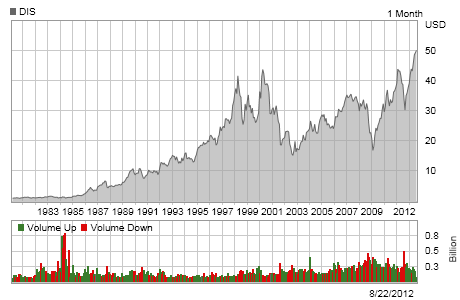
\includegraphics{DisneyChart.png}      %-- include image file named as "disneychart.png" 
   \caption{This is the figure's caption -- Disney stock chart}
    \label{fig:disneystock}
\end{comment}


\begin{comment}
 \item \citeA{kartch:2000:ERA} compared reaction times...
 \item In a recent study of reaction times \cite{kartch:2000:ERA}...
 \item In \citeyearNP{kartch:2000:ERA}, \citeauthor{kartch:2000:ERA} compared reaction times...
 \item \shortciteA{fedkiw:2001:VSO} compared reaction times... 
 \item In a recent study of reaction times \cite{fedkiw:2001:VSO}...
 \item In \citeyearNP{fedkiw:2001:VSO}, \shortciteauthor{fedkiw:2001:VSO}, compared reaction times...
\end{comment}



\section{Research Objectives}
\label{sec:researchobjectives}

\subsection{General Objective}
\label{sec:generalobjective}

To create a system that stores and retrieves useful information from digital images of paper forms to provide a fast and convenient way for viewing the information on a screen.   


\subsection{Specific Objectives}
\label{sec:specificobjectives}

%
%  \begin{comment} ... \end{comment} is used for multiple lines of comment
%



\begin{comment}

This subsection is an elaboration of the general objective.  It states the specific steps that must be undertaken to accomplish the
general objective.  These objectives must be specific, measurable, attainable, realistic, time-bounded.  Each specific objective may
start with ``to design/survey/review/analyze''

Studying a particular programming language or development tool (e.g., to study Windows/Object-Oriented/Graphics/C++ programming) to 
accomplish the general objective is inherent in all thesis and, therefore, must not be included here.


%
% IPR acknowledgement: the following sentences and examples are from Ethel Ong's slides 
%     on Research Objectives
%

How to formulate your research objectives:
1. Identify what research steps do you need to perform to achieve your general objective.
2. Identify the questions that must be answered for you to achieve your general objective.
    Thereafter, convert these questions into action statements


Example #1:

Research Question:
  What are the general features of a web-based learning environment?

Specific Objective:
   To review existing web-based learning environment that teaches language learning for children


Example #2:

Research Question:
   How will you represent commonsense knowledge for use by computer systems?

Specific Objective:
   To identify knowledge representation approaches used by existing story generation systems

Example #3:
Research Question:
   What types of storytelling knowledge are needed to generate stories?

Specific Objective:
    To identify the different types of storytelling knowledge used in generating stories

Example #4:
Research Question:
    What machine learning approaches will you utilize?

Specific Objective:
    To determine existing machine learning algorithms [that can be used in training the computer system to detect cyberbullying cases] 

Example #5: Research Question:
    How will your research output be evaluated?

Specific Objective:
    To define evaluation metrics for validating the accuracy of the translation

\end{comment}

%
%  The following are example specific objectives; replace them with your own 
%

\begin{enumerate}
   
   \item To provide a modified version of the current medical examination form that will be more appropriate in the process.
   \item To implement an algorithm that extracts the medical examination form from the mobile captured image.
   \item To prepare the extracted image for segmentation by implementing a dewarping algorithm.
   \item To implement an algorithm that extracts and identifies the multiple sections of the form.
   \item To extract the data on the identified sections as strings.
   \item To create a database that stores extracted strings of the form.
   
\end{enumerate}


\section{Scope and Limitations of the Research}
\label{sec:scopelimitations}

The study focuses on the segmentation of specific types of forms and its implementation will cover selected image processing algorithms from reviewed studies. Currently, medical examination forms exists for the use of the GetBetter system. These forms are to be modified to be more compatible with the algorithms to be used. The test images that will be used in the study will mainly be a variety of mobile captured images of the modified forms.

The performance of image segmentation techniques depend heavily on the quality of the image. It is important to note that the quality of the image may vary depending on the hardware used to take the picture, on the physical condition of the paper form and on the circumstances the image was taken. Because of this variance, it cannot be guaranteed that image segmentation process will work for all kinds of images and conditions, however an algorithm that will work under the worst condition will be employed to guarantee maximum effort and performance instead. For the purpose of GetBetter, the test images in this study will be those which are captured on a Samsung tablet since that is what is currently being used.


\begin{comment}

%
% IPR acknowledgement: the sentences inside this comment are from Ethel Ong's slides on Scope and Limitations of the Research
%
Generally, one paragraph should be allotted for each of your research objectives.

Each paragraph contains a brief overview of the concept/theory and the purpose of doing the associated objective.

Each paragraph also includes a description of the scope/limitation of your study.

* Please refer to the slides for examples.

\end{comment}


\section{Significance of the Research}
\label{sec:significance}

People are growing to be more dependent on technology and because of this almost everything is becoming digital including physical documents. Providing a way to make these documents presentable and accessible on various devices is now an important matter.

The GetBetter Tele-Diagnosis System lacks the functions which can support the transformation of the forms in images into a better digital representation of the form. Currently the system does not provide an interface that allows doctors to obtain sections of a patient’s medical examination form separately. Providing functions that will allow a systematic approach in the diagnosis process is a step further in enabling the doctors to become more productive and the system more convenient.

The resulting database of images which contain information about the patients can then be used by an Optical Character Recognition system to replace the images with actual values represented as strings or numbers. This will produce a more comprehensible information that the users and system can utilize.

%
% IPR acknowledgement: the following list of items are from Ethel Ong's slides on Significance of the Research
%
\begin{comment}
\begin{itemize}
\item  What is the relevance of your work to the computer science community? 

\begin{itemize} 
\item What will be your technical contributions, in terms of algorithms, or approaches, or new domain? 
\item What is your value-added compared to existing systems? 
\end{itemize}

\item What will be your contributions to society in general? 
    \begin{itemize}
      \item Who will benefit from your system? 
      \item Who are your target users and how will this system benefit them? 
   \end{itemize}
\end{itemize}

If applicable, describe possible commercialization and/or innovation in your research.
\end{comment}


